% !TeX spellcheck = en_US
\section{Traditional Feature-Based \ac{ser}}


\subsection{Feature Extraction}

The first step in a traditional approach is feature extraction to transform raw audio data into a set of informative features that can capture key characteristics of the signal.

In this regard, the widely-used Librosa toolkit was employed to extract various audio features, from the audio files of the \ac{iemo} dataset, and subsequently, they were processed using statistical metrics. The extracted features and associated metrics are summarized in Table \ref{table:extractedFeat}, with a total of 327 extracted features.

\begin{table}[h]
	\centering
	\caption{Extracted audio features and the statistical functions applied.}
	\label{table:extractedFeat}
	
	\begin{tabular}{@{}cc@{}}
		\toprule
		Audio Features & Statistical Functions \\
		\midrule
		&  \multirow{10}{*}{\begin{tabular}{@{}c@{}}Minimum\\Mean\\Maximum\\Median\\25th percentile\\75th percentile\\Spikes\footnotemark[1]\\Variance \\Standard Deviation\\Sum\\Kurtosis\footnotemark[2]\\Skew\footnotemark[2]\end{tabular}} \\
		\acp{mfccs} 1 - 21 & \\
		Mel Spectrogram & \\
		Root-Mean-Square & \\
		Chromagram & \\
		Spectral Centroid & \\
		Spectral Contrast & \\
		Spectral Bandwith & \\
		Roll-Off Frequency & \\
		Tonnetz & \\
		Zero-Crossing Rate & \\
		& \\
		\bottomrule
		\multicolumn{2}{l}{\footnotemark[1]\footnotesize{Custom function detailed on the feature selection subsection \ref{spikes:metric}.}} \\
		\multicolumn{2}{l}{\footnotemark[2]\footnotesize{Only for the \acp{mfccs}.}} \\
	\end{tabular}
\end{table}

\subsection{Feature Analysis}

An important task following feature extraction is analyzing and interpreting the extracted data to gain a deeper understanding of the audio signals and the features that describe them.

\subsubsection{Audio Features Visualization}

In this process, we visually analyzed and interpreted the features' data by graphically representing each feature from an audio segment. The figures in Section \ref{app:1} of the appendix demonstrate some of the graphics we used to visualize the features.

\subsubsection{Spikes Metric}
\label{spikes:metric}

Initially, wave plots were observed, and we noted consistency in the number of high values. For this reason, we created a custom metric that calculates those high values, which we called "spikes", from the features' data.

In Figure \ref{fig:zcrSpikes}, it is possible to visualize the zero crossing rates' wave plots in different emotions. The horizontal line represents the threshold that we considered, any value above was considered to be a spike, which is annotated with red dots in the graphic. The threshold used was manually tested and obtained decent consistency of the number of spikes, within an emotion, by using the mean value of the feature plus 2\% of the standard deviation. To account for different-length audio signals, it was also divided the number of spikes to the total length of the data, as the Code Snippet \ref{spikes:code} demonstrates. Consequently, this metric was also tested and applied to every other audio feature.

\begin{figure}[H]
	\centering
	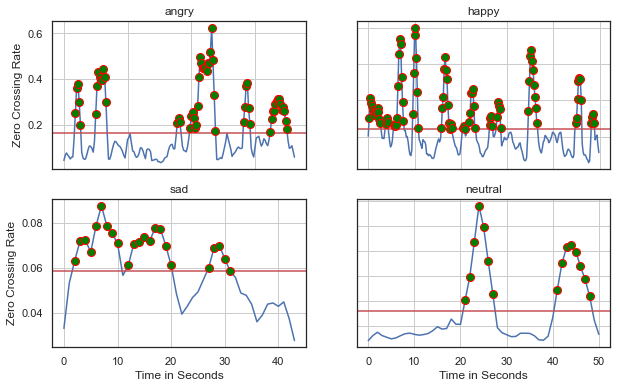
\includegraphics[width=.7\textwidth]{figs/4_1_traditional/zcr_waveplot_spikes.png}
	\caption{Zero crossing rate wave plot annotated with spikes.}
	\label{fig:zcrSpikes}
\end{figure}

\begin{listing}[H]
	\begin{minted}{python}
def spikes(data):
	mean = np.mean(data)
	std = np.std(data)
	threshold = mean + np.abs(std) * 2 / 100
	num_spikes = 0
	for value in data:
		if value >= threshold:
			num_spikes += 1
	return num_spikes / len(data)
	\end{minted}
	\caption{Python code for calculating the spikes metric.}
	\label{spikes:code}
\end{listing}



\subsubsection{Bar Plots}

Furthermore, bar plots were useful for viewing the overall extracted features' data plainly and quickly, and to understand the numeric values of each feature and metric used on it.

For example, figure \ref{fig:melBarPlot} shows clear differences in the mean values for some metrics used on the Mel Spectrogram. Other bar plots are presented in the appendix \ref{app:2}.

\begin{figure}[H]
	\centering
	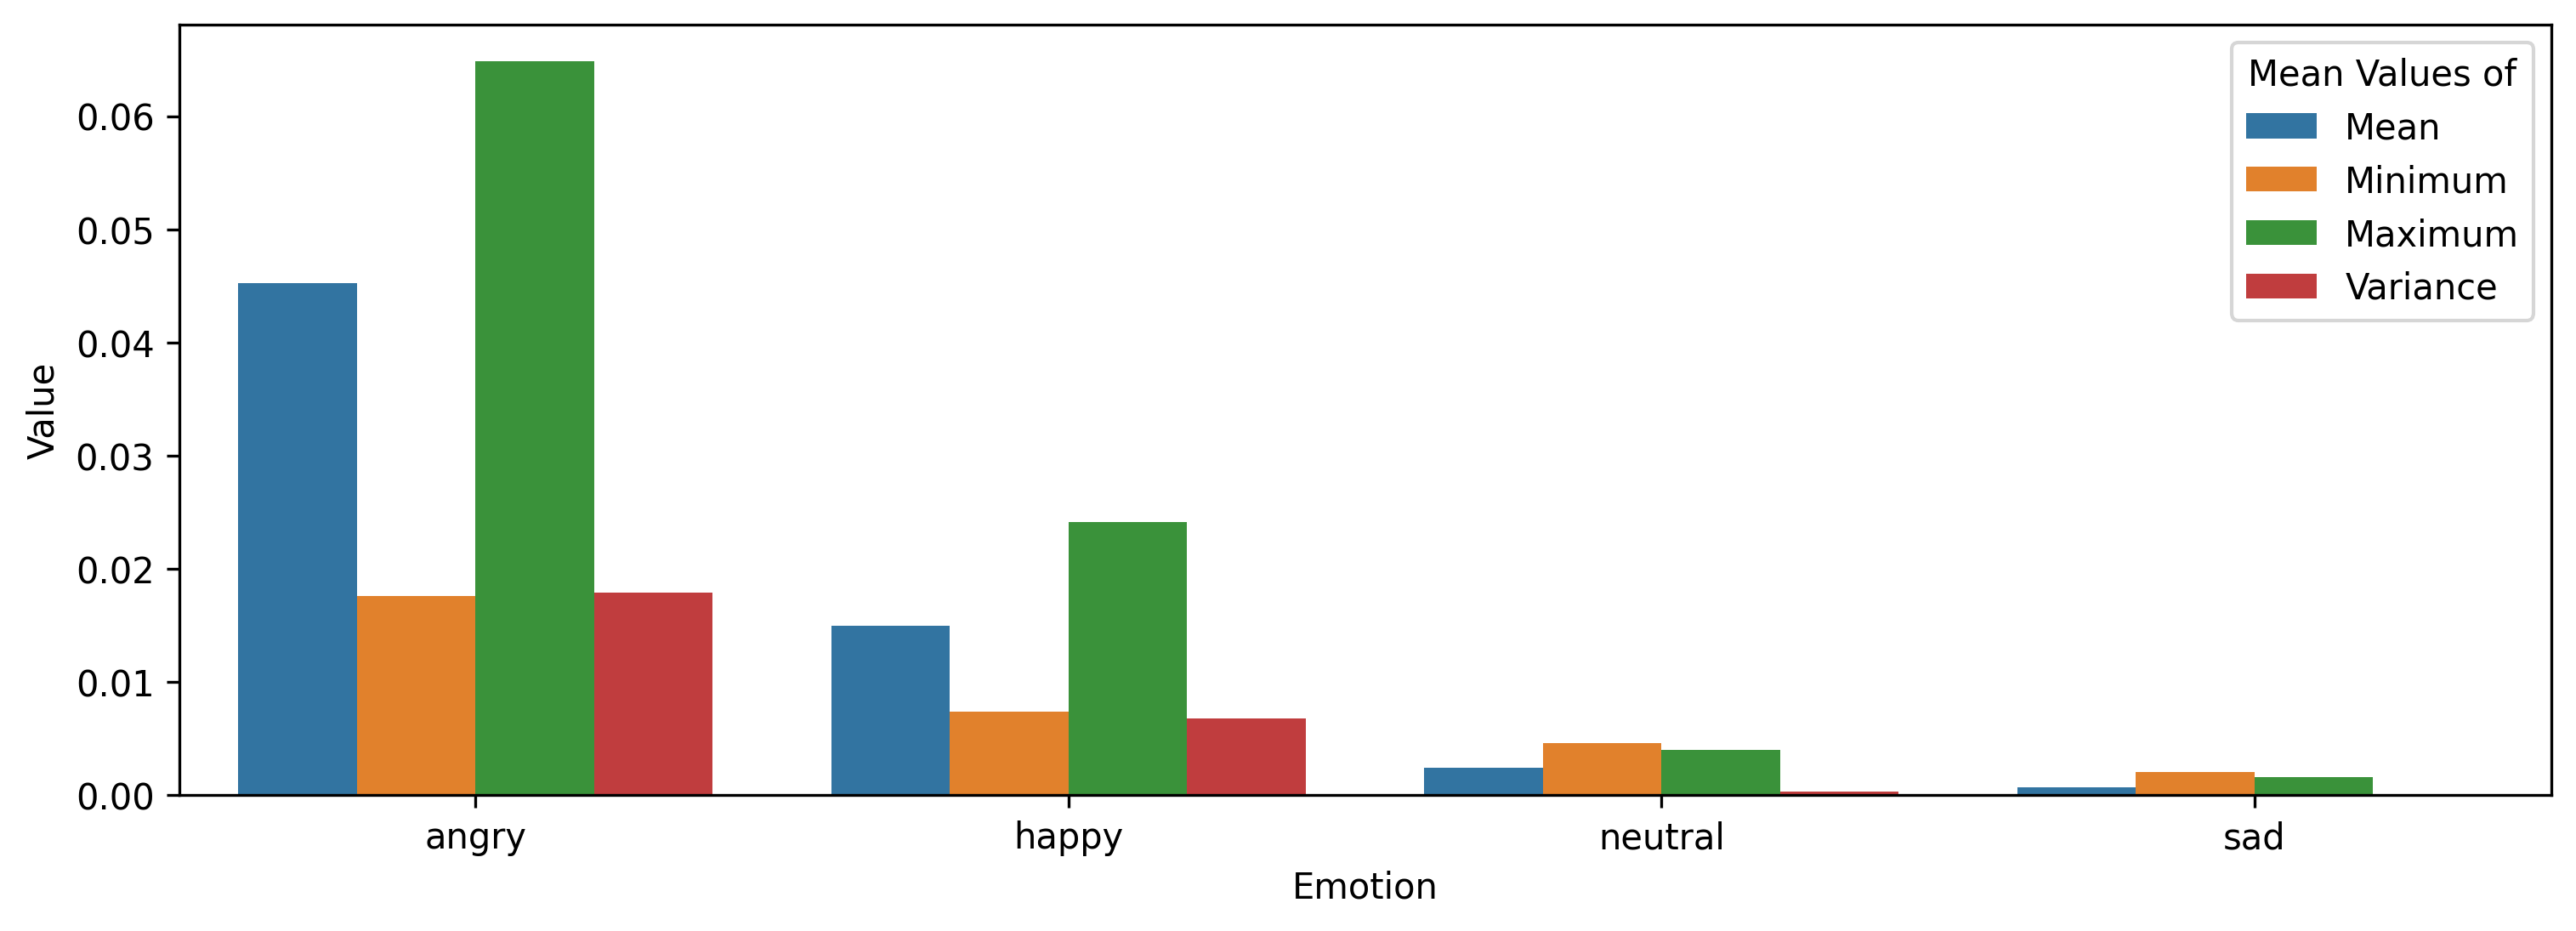
\includegraphics[width=\textwidth]{figs/4_1_traditional/meanFeatBarPlot.png}
	\caption{Bar plots mean for metrics used on the mel spectrogram feature.}
	\label{fig:melBarPlot}
\end{figure}


\subsubsection{Wave Plots with Surrounding Areas}

During the feature study process, it was observed the wave plots of some features surrounded by a small area above and below the original wave (defined through a selected threshold). This was done to corroborate how well the feature describes different emotions. A high degree of overlap between surrounding areas of a feature, for a given emotion, could indicate that the feature  has consistent values and is relevant for identifying that emotion.

Figure \ref{fig:zcrAreaOnly1} is an excerpt of the figure \ref{fig:zcrArea} in the appendix \ref{app:3}, and it demonstrates an example of this analysis for the zero crossing rate with 5 different subjects on the same sentence for the anger emotion. From this graphic, it was observed that there is an overlap between the surrounding areas for each emotion, which allows us to conclude that the feature has utility for describing each emotion. However, due to the different lengths of each audio segment, it is ambitious to guarantee this conclusion.

\begin{figure}[H]
	\centering
	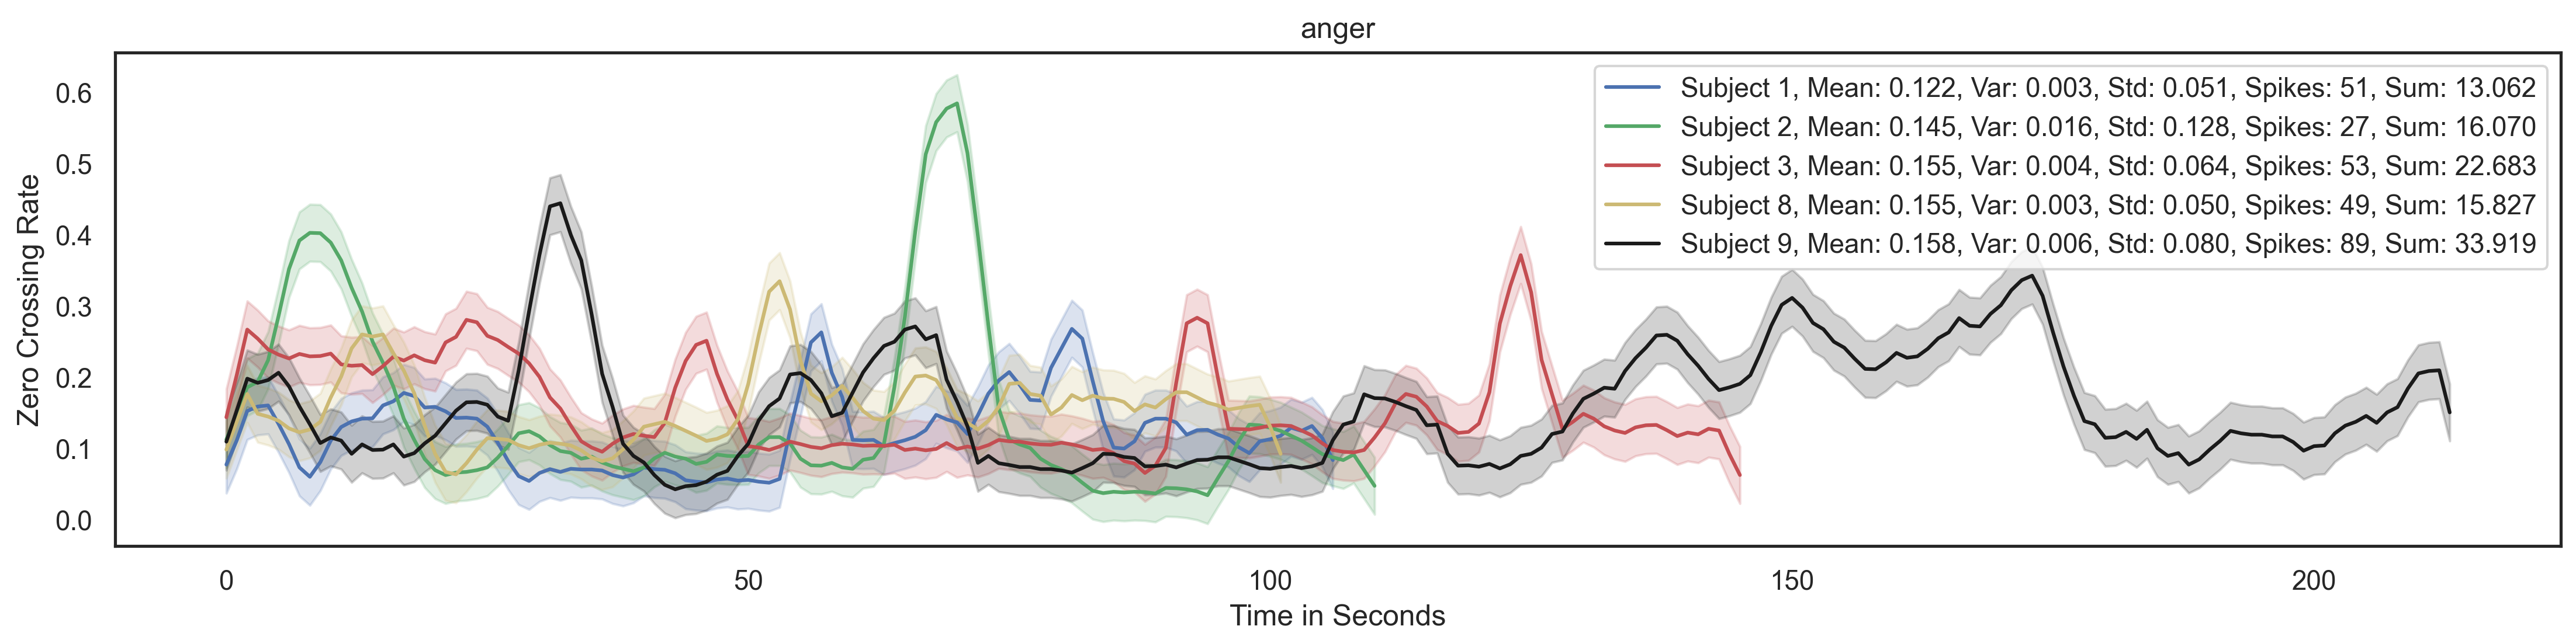
\includegraphics[width=1\linewidth]{figs/4_1_traditional/zcrAreaOnly1.png}
	\caption{Zero crossing rate wave plot with a surrounding area of five male subjects for the same utterance with the anger emotion.}
	\label{fig:zcrAreaOnly1}
\end{figure}

This same idea can also be used to determine whether a feature is favorable for creating a distinction between different emotions, which is naturally useful for the problem of classifying emotions. The conclusion can be drawn by observing the opposite of the previous case. If the areas around the feature, on different emotions, do not heavily overlap, it may be an indicator that the feature can be able to discriminate emotions. Figure \ref{fig:zcrAreaSameSubj} displays six zero crossing rates of one subject saying the same sentence but expressing different emotions. As previously mentioned, since audio lengths are different, it is challenging to draw a direct and well-founded conclusion.

\begin{figure}[H]
	\centering
	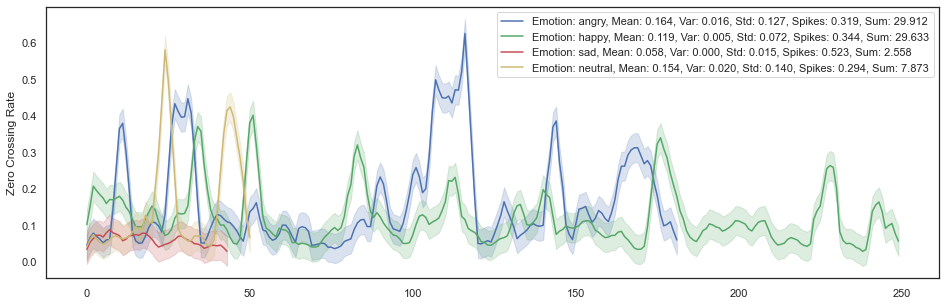
\includegraphics[width=.8\linewidth]{figs/4_1_traditional/zcr_male_same_subject.png}
	\caption{Zero crossing rate wave plots with a surrounding area of a single male subject and sentence for all different emotions.}
	\label{fig:zcrAreaSameSubj}
\end{figure}

Overall, this approach of surrounding wave plots with areas provided us valuable insight into the ability of a feature to describe and distinguish emotions, though it is limited by the varying lengths of audio segments.

\subsubsection{Variation Plots}

Another graph made was a variation plot, to perceive the differences in the features' values, across several audios for the same emotion. Figure \ref{fig:zcrMeanVar} shows an example of this type of plot for the mean zero crossing rate value across 50 speech utterances for all emotions. Other examples of this type of graphic are also in the appendix \ref{app:4}.

\begin{figure}[H]
	\centering
	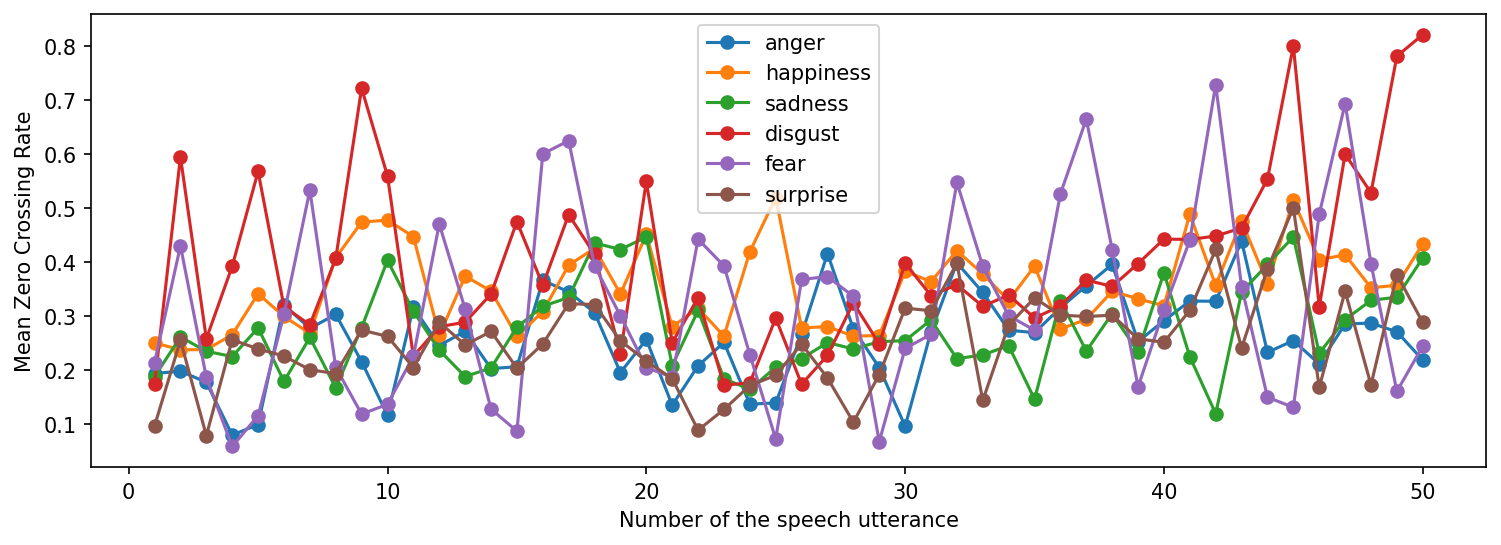
\includegraphics[width=\linewidth]{figs/4_1_traditional/meanZCRVar.png}
	\caption{Zero crossing rate mean values variation plot along 50 audios of speech utterances for all emotions.}
	\label{fig:zcrMeanVar}
\end{figure}

A common observation for most extracted feature plots was that the values were not consistent across multiple audio segments for the same emotion. However, the number of audio segments used in this study was relatively low (only 50) to observe big variability changes, but increasing the number of audio segments would also make it more challenging to observe such variability through a simple visual inspection.

\subsubsection{Box Plots}

Finally, we employed box plots to visualize the distribution of the features on different subjects, as well as to compare the values for each emotion. An example of this type of plot is shown in Figure \ref{fig:zcrMeanBoxPlot}, which displays the mean zero crossing rate feature for all emotions and different subjects. 

\begin{figure}[H]
	\centering
	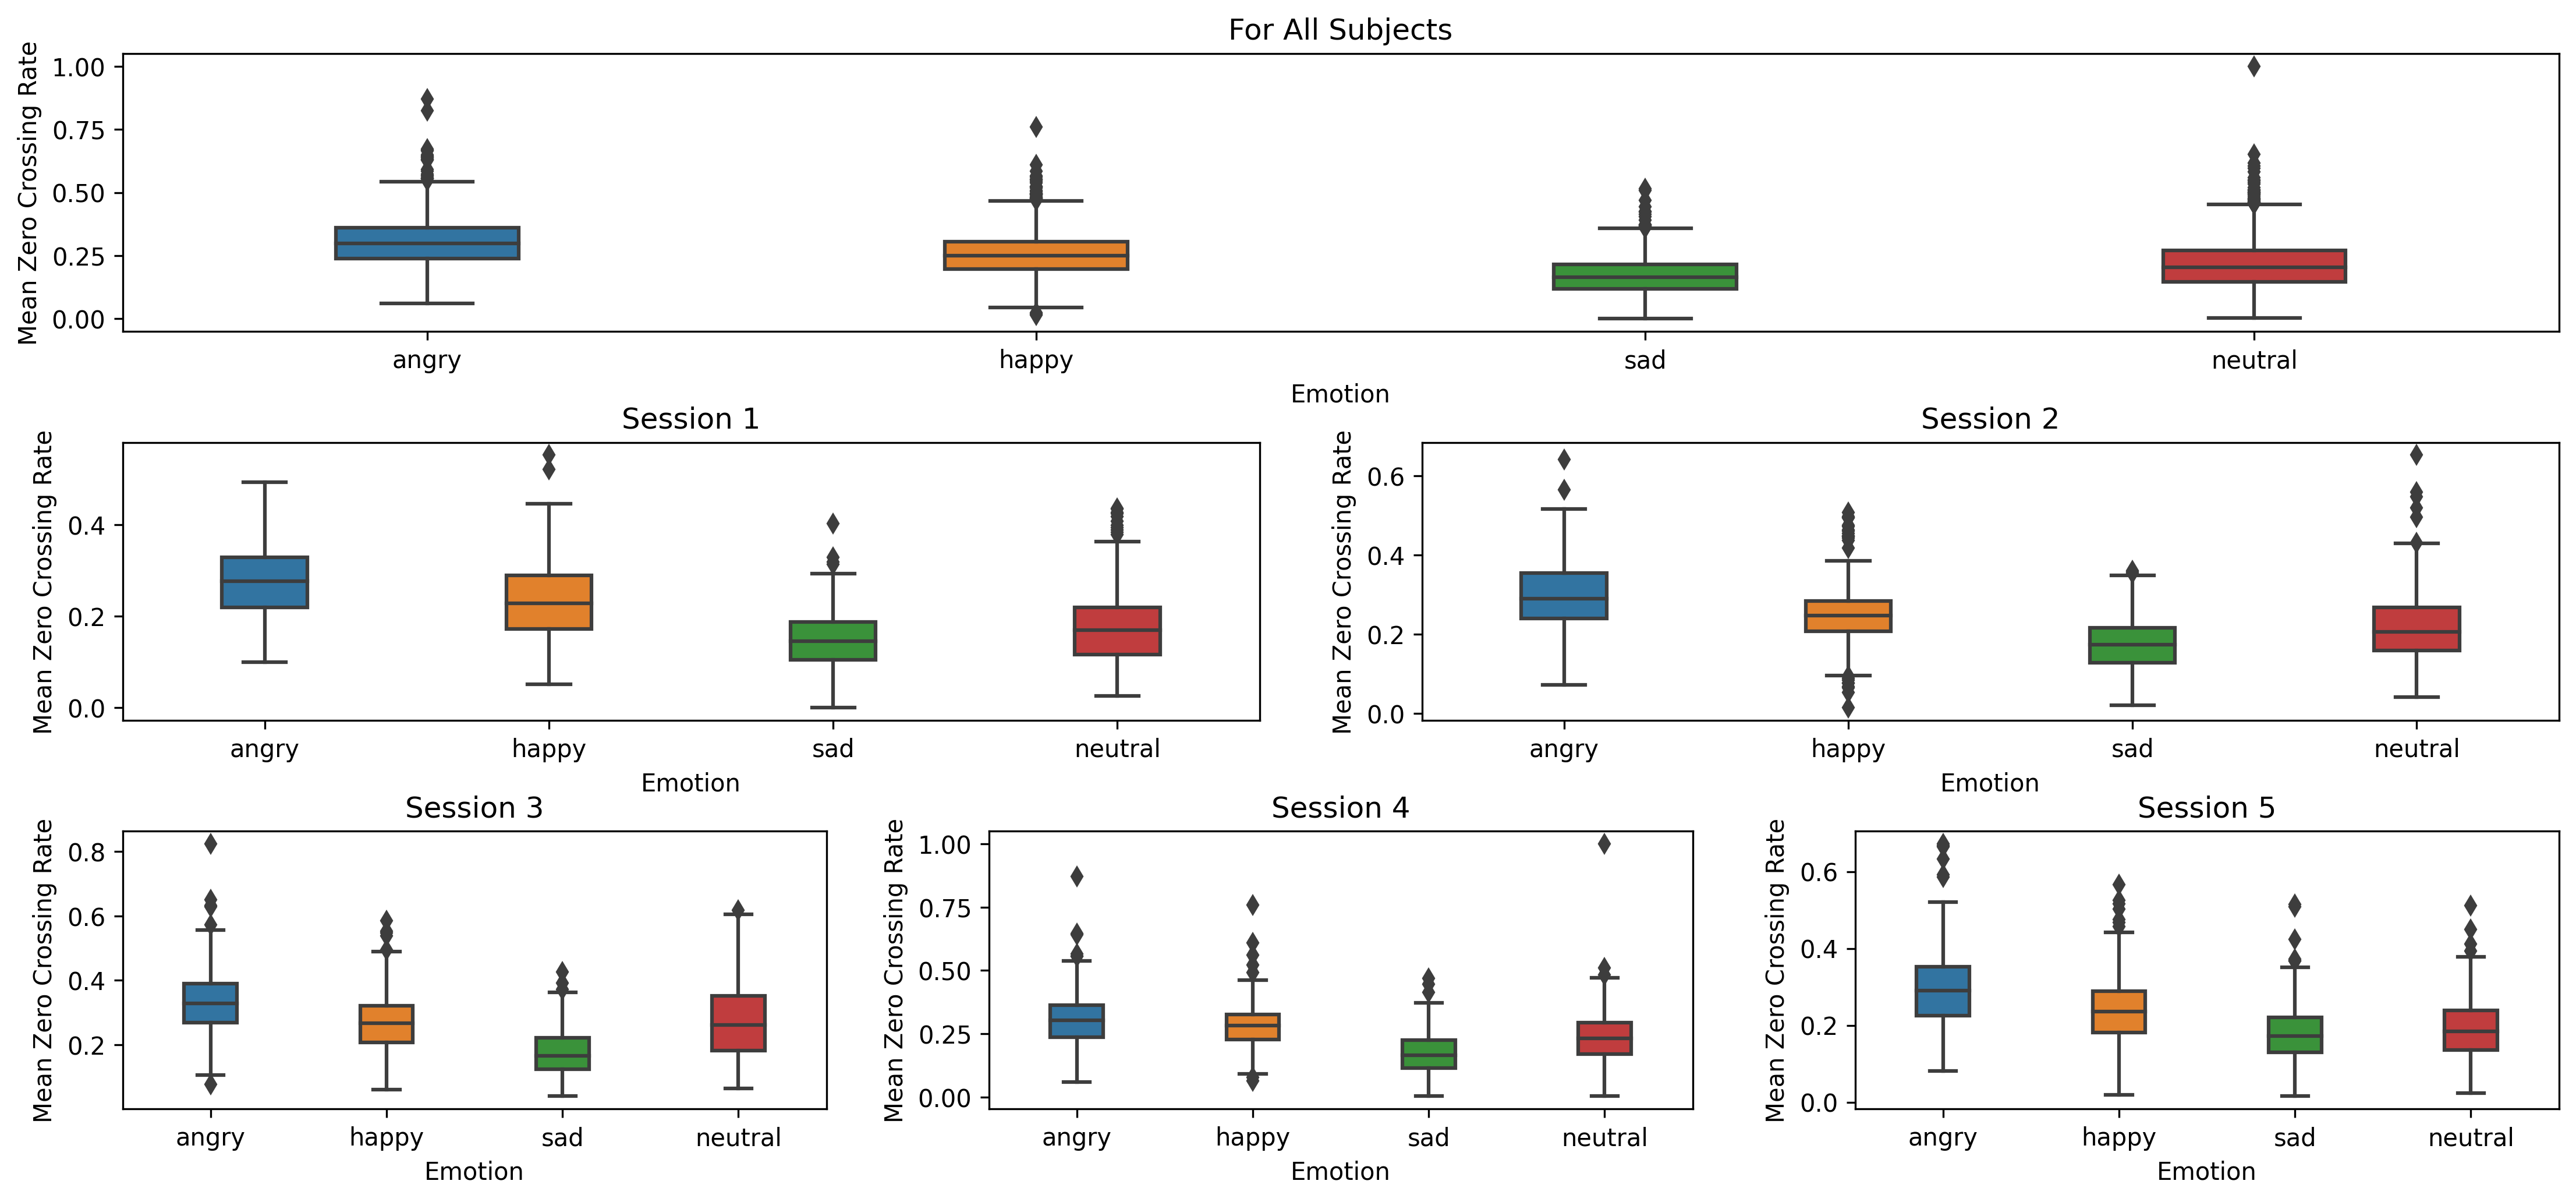
\includegraphics[width=\linewidth]{figs/4_1_traditional/mean_zcr_box_plot.png}
	\caption{Zero crossing rate mean values box plot for all emotions and different subjects.}
	\label{fig:zcrMeanBoxPlot}
\end{figure}

The primary purpose of using these plots was to provide a simple and intuitive representation of each feature. By comparing the values across all subjects or a selected few, any noticeable differences in feature values for each emotion could be easily perceived.

\subsection{Feature Selection}

After the process of feature analysis, the next step in \ac{ser} development is feature selection. Feature selection is a technique to choose a subset of the original set of features that are most relevant for the given task. The process of feature selection is aimed to improve the accuracy of the model and reducing the problem's complexity by removing redundant or irrelevant features. 

The objective is to choose a smaller set of features that retain enough information for good classification performance while being computationally efficient. Hence, a smaller subset of features that can provide effective classification results is preferred over the larger set of features that may be computationally expensive and redundant.

\subsubsection{\acl{cfs}}

Correlation among our extracted features is common since many of them use the same audio descriptor but with a different metric applied to them. Therefore, a correlation matrix for all 327 extracted features was calculated using the Pearson method, presented in figure \ref{fig:allAudioFeat}.

A \ac{cfs} was performed by selecting every pair of features with a Pearson correlation coefficient absolute value of 0.6 or above, then it was removed the feature with the highest average correlation value with all the other features. This process resulted in the elimination of 229 features, leaving 98 features for subsequent analysis. The correlation matrix after the feature selection process is presented in figure \ref{fig:highAudioFeat}.

\begin{figure}[H]
	\begin{subfigure}{.5\textwidth}
		\centering
		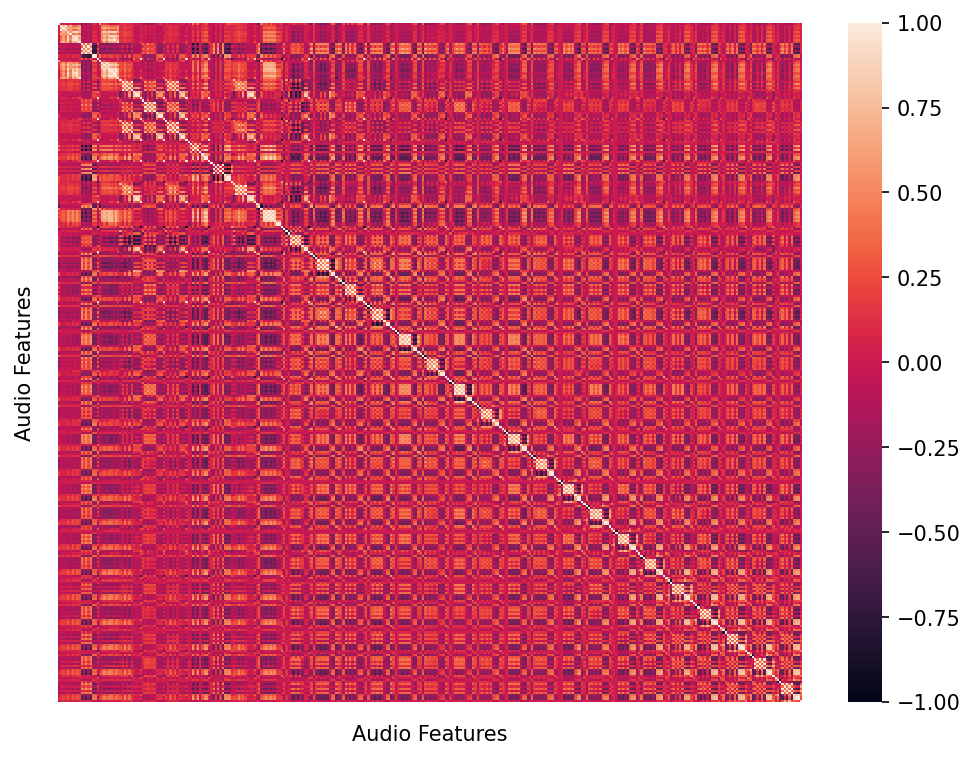
\includegraphics[width=\linewidth]{figs/4_1_traditional/allCorrMatrix.png}
		\caption{Correlation matrix of all the features.}
		\label{fig:allAudioFeat}
	\end{subfigure}%
	\begin{subfigure}{.5\textwidth}
		\centering
		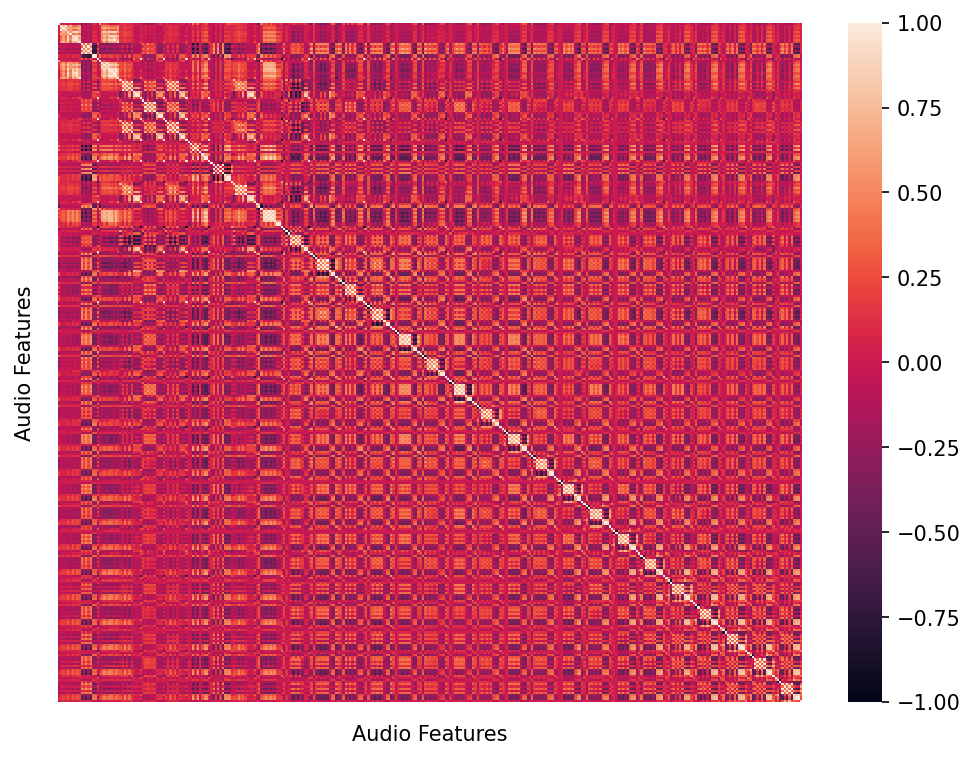
\includegraphics[width=\linewidth]{figs/4_1_traditional/highCorrMatrix.png}
		\caption{Correlation matrix after \ac{cfs}.}
		\label{fig:highAudioFeat}
	\end{subfigure}
	\caption{Audio features' correlation matrices before and after \ac{cfs}.}
\end{figure}

\subsubsection{Selecting an Initial Classifier}

Along this process, it became necessary to choose a model to be used in computationally expensive feature selection methods. Consequently, several estimators were tested for their performance in classifying emotions.

To this end, we conducted 5-fold \ac{cv} and compared the mean and standard deviation accuracies of all folds, as well as the total execution time for various classifiers using default parameters from the scikit-learn library \cite{pedregosa2011scikit}. The input given to the models is the set of features obtained after \ac{cfs}, as shown in Table \ref{tab:modelsPerformance}.

\begin{table}[H]
	\caption{Performance of various classifiers in 5-fold \ac{cv} using the features obtained after \ac{cfs}.}
	\centering
	\label{tab:modelsPerformance}
	\begin{tabular}{lrrr}
		\toprule
		Classifiers &  Accuracy & Training Time (s) \\
		\midrule
		\ac{xgb}                &        0.617$\pm$0.013  & 17.628 \\
		\ac{rf}                &        0.578$\pm$0.010  &  7.451 \\
		Ridge                  &        0.565$\pm$0.014  &  0.078 \\
		Extra Trees            &        0.561$\pm$0.005  &  1.831  \\
		AdaBoost               &        0.520$\pm$0.008  & 12.205  \\
		C-Support Vector       &        0.504$\pm$0.018  &  5.081 \\
		DecisionTree           &        0.450$\pm$0.022  &  1.886 \\
		Multi-layer Perceptron &        0.446$\pm$0.027  &  4.821 \\
		\bottomrule
	\end{tabular}
\end{table}

Based on the evaluation results, the \ac{rf} classifier was chosen for further analysis. This model exhibited the second-best average accuracy across the 5 folds, however, it was much faster than the \ac{xgb} to train. Therefore, \ac{rf} was the selected model for performing computationally expensive feature selection methods.


\subsubsection{Backwards Selection}

In the pursuit of completing the feature selection process, a sequential feature selection with backward propagation was employed. This method involves performing a 5-fold \ac{cv} with the previously selected \ac{rf} classifier, using all features except one, and then removing one feature based on the lowest mean accuracy of the 5 folds. This iterative process continues until only one feature remains.

A method was then developed to select the furthest and highest accuracy. This method resembles the standard maximum, but it multiplies the maximum value by a threshold value of $0.99$ so that it can find close to the maximum values that have more features removed, creating a balance between accuracy and the number of features. Figure \ref{fig:backProp1} displays the mean accuracies obtained at each step and the chosen furthest highest accuracy.

\begin{figure}[H]
	\centering
	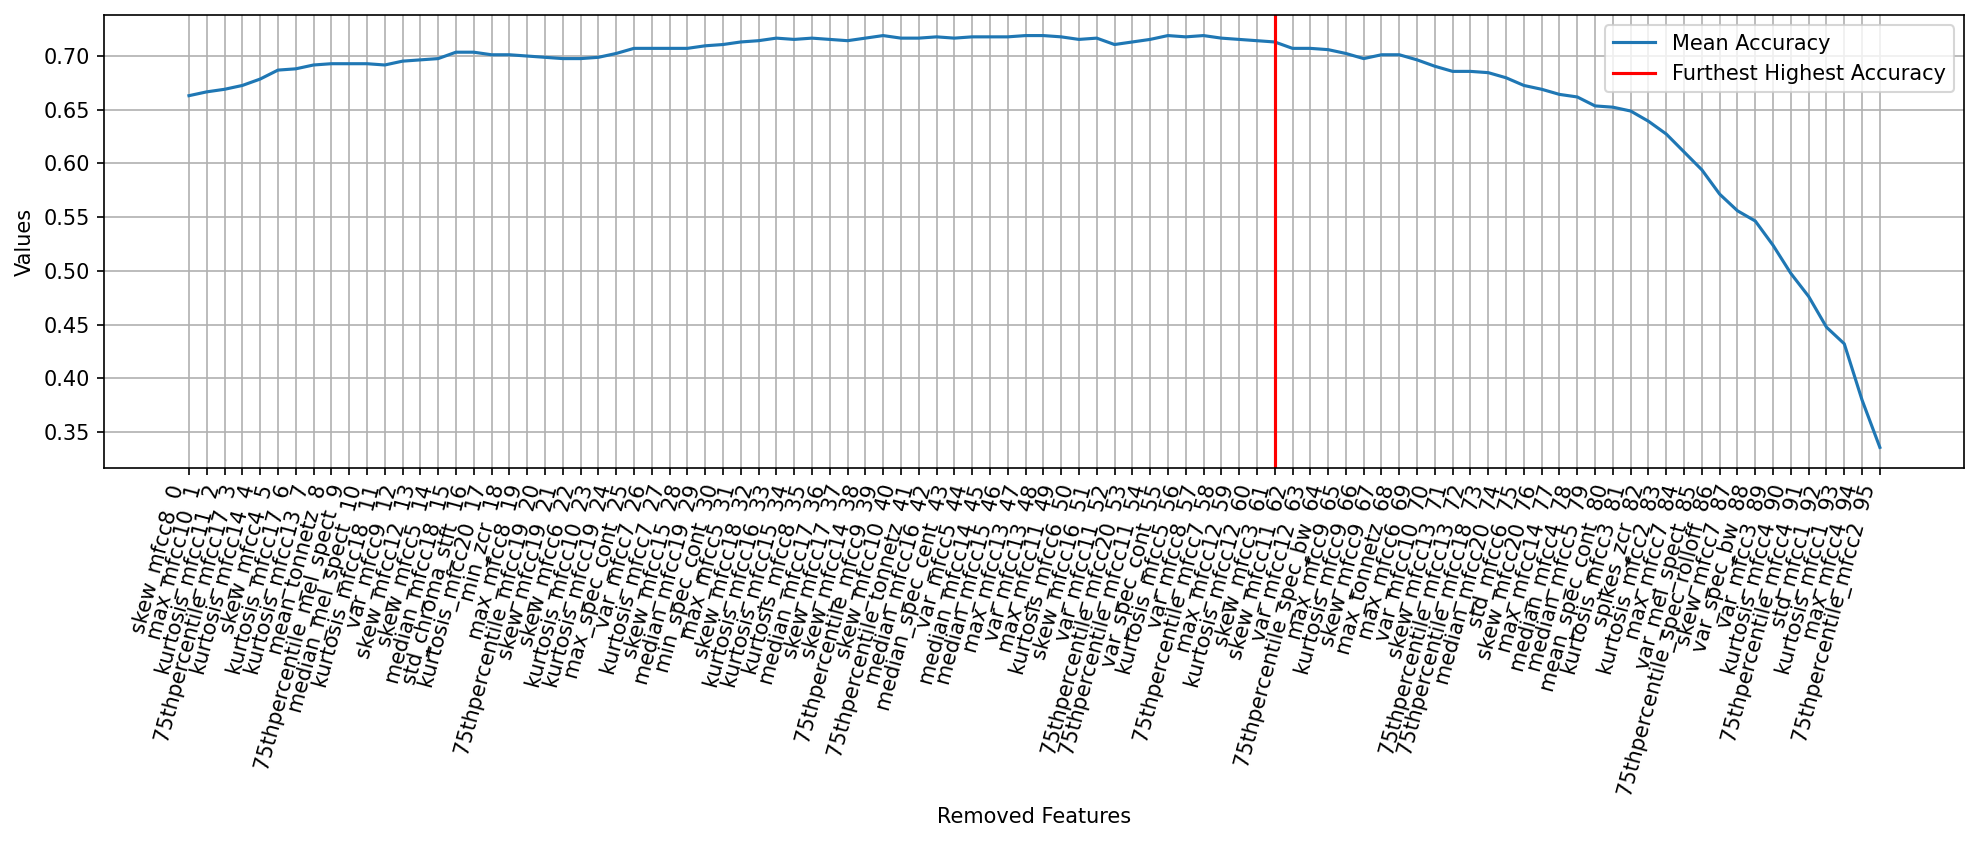
\includegraphics[width=1\linewidth]{figs/4_1_traditional/backProp1.png}
	\caption{Sequential feature selection with backward propagation using the mean accuracy as the selection criteria.}
	\label{fig:backProp1}
\end{figure}

This process led to the elimination of 65 features from the initial set of 98 obtained after \ac{cfs}, leaving a total of 33 features, as shown in Table \ref{tab:selectedFeat}.

\begin{table}[H]
	\caption{Final set of the 33 selected features.}
	\centering
	\label{tab:selectedFeat}
	\resizebox{\textwidth}{!}{%
		\begin{tabular}{ll}
			\toprule
			Metric & Audio Features \\
			\midrule
			Spikes & Mel-Spectrogram, Chromagram, Zero Crossing Rate, MFCC-6, MFCC-16, MFCC-19 \\
			Mean & Spectral Bandwidth, MFCC-13, MFCC-15, MFCC-17, MFCC-19, MFCC-20 \\
			Maximum & Spectral Bandwidth, MFCC-5, MFCC-7, MFCC-10, MFCC-11 \\
			Variance & Mel-Spectrogram, MFCC-1, MFCC-3, MFCC-5, MFCC-8 \\
			Kurtosis & MFCC-12, MFCC-17, MFCC-18 \\
			25th Percentile & Chromagram, Root Mean Square \\
			75th Percentile & MFCC-7, MFCC-11 \\
			Sum & MFCC-10, MFCC-12 \\
			Median & MFCC-5 \\
			Min & Zero Crossing Rate \\
			\bottomrule
		\end{tabular}
	}
\end{table}



\subsubsection{Feature Selection Evaluation}

To assess the feature selection quality on the development dataset, we trained and evaluated the predictions of a \ac{rf} Classifier model with different sets of features, using accuracy as the evaluation metrics. The results are presented in Table \ref{tab:acc}. Additionally, we plotted the confusion matrices of the predictions, which can be found in the appendix \ref{confusionMatrices}.

\begin{table}[H]
	\caption{\ac{rf} 5-fold \ac{cv} evaluation metrics using different sets of features.}
	\centering
	\label{tab:acc}
	\begin{tabular}{lrrr}
		\toprule
		Feature Selection Method & N.º of Features & Accuracy & Training Time (s)\\
		\midrule
		None & 327 & 59.14$\pm$0.68 & 15.34 \\
		\ac{cfs} & 98 & 57.87$\pm$1.07 & 7.89 \\
		\ac{cfs} \& Backward Selection & 33 & 59.12$\pm$1.05 & 4.29\\
		\bottomrule
	\end{tabular}
\end{table}

The results of the feature selection techniques have shown that while there may be a small loss of accuracy between the initial set of extracted features and the set obtained after \ac{cfs}, the model can achieve comparable accuracy while using only around 70\% of the original set. Moreover, applying backward selection to the remaining 98 features yields optimal results by maintaining the accuracy and reducing the original feature set by approximately 90\%.

By using these feature selection techniques, we managed to remove redundant and irrelevant features, which also decreases the models' complexity and size, providing several practical benefits for its implementation and interpretation.


\subsection{Classifiers Evaluation and Selection}

\subsubsection{Evaluation Strategy}

Evaluating a model is an essential step, since a wrongful evaluation may lead to deception in terms of the results obtained. It should be uniform for every model, and, it should be as meaningful as possible to the classification objective.

For the reasons above and because it was the most recurred method in the \ac{sota} research, it was decided to utilize 5-fold stratified \ac{cv} with an 80-20 train-test split, which provides more fairness to model comparisons. In terms of metrics, we decided to calculate the testing folds averages accuracy, macro-f1 score, precision, recall, and \ac{mcc}.

Accuracy is a basic metric to evaluate the model's performance that measures the proportion of correctly classified samples. Precision measures the proportion of true positives among all samples predicted as positive by the model. Recall indicates how many of the actual positive samples are correctly identified by the model. The macro-f1 score takes into account both precision and recall to provide a more balanced measure of performance for imbalanced datasets. It calculates the harmonic mean of precision and recall. \ac{mcc} is a correlation coefficient between the true labels and the predicted labels. It measures how well the model's predictions match the true labels, and ranges from -1 (perfect disagreement) to +1 (perfect agreement), 0 being no agreement at all, which means the predictions were random. A \ac{cm} of the predicted and real labels was also plotted, since it provides helpful insights, not only into the errors being made by the classifier but also, the types of errors occurring.

\subsubsection{Machine Learning Models}

To develop the most effective speech emotion recognition model, a variety of automatic machine learning techniques were employed in the study. Two different \ac{aml} techniques were employed to search for the best models. One such technique was the Auto-SKLearn ensemble \cite{feurerneurips15a}. This technique searches for the best models and ensembles by exploring a vast space of possible algorithms and hyperparameters using a meta-learning approach. After training and obtaining the ensemble model, the most influential classifiers of the ensemble were identified and taken into account for further exploration individually.

Another \ac{aml} technique, AutoKeras \cite{jin2019auto}, was applied to create a \ac{cnn} model, which we also used to create another model by combining it with an \ac{lstm}. So, in addition to the previous classifiers, two deep-learning models were also evaluated.

Based on this, we explored multiple classifiers for \ac{ser} and tested several hyperparameters for each model to find the most optimal results, including:

\begin{enumerate}
	\item \ac{rf}: A popular decision tree-based ensemble method that trains multiple decision trees on different subsets of the dataset and outputs the mode class predicted by the trees.
	
	\item Balanced \ac{rf}: A variant of the \ac{rf} that addresses class imbalance by undersampling the subsets provided to train each tree.
	
	\item \ac{xgb}: A gradient boosting model that uses decision trees as base learners. Each tree is trained using the negative gradient of the loss function concerning the prediction of the previous iteration. This means that each subsequent tree corrects the errors of the previous ones, leading to a more accurate final prediction.
	
	\item AdaBoost: Short for Adaptive Boosting, it is a boosting algorithm that combines multiple weak classifiers into a strong classifier by iteratively adjusting the weights of incorrectly classified instances. At each iteration, a new weak classifier is trained, and its weight is added to the ensemble based on its accuracy. The final prediction is then made by summing the weighted predictions of all the weak classifiers.
	
	\item Histogram Gradient Boosting: An ensemble model that combines gradient boosting with a histogram-based approximation of decision trees, which improves performance on large datasets. It splits data into histograms based on their values instead of splitting features to create decision trees.
	
	\item \ac{svm}: A linear or nonlinear model that finds the best boundary separating data into different classes by maximizing the margin between the classes.
	
	\item Ridge:A linear model with L2 regularization that minimizes the sum of squared residuals between the predicted and actual values.
	
	\item Linear Discriminant Analysis: A statistical approach that finds a linear combination of features to maximize the separation between classes by modeling the distribution of the data in each class.
	
	\item \ac{cnn}: A neural network commonly used for image classification tasks. It applies filters to the given input through convolutional layers to extract different features, passes these features through pooling layers to reduce dimensionality, and produces the final output label using fully connected layers.
	
	\item \ac{cnn} + \ac{lstm}: A hybrid deep learning architecture that combines the strengths of convolutional and recurrent neural networks, allowing for both local and temporal feature extraction from the data.
\end{enumerate}



\subsubsection{Results and Conclusions}

Having chosen a set of classifiers, we then applied our evaluation strategy on the \ac{iemo} dataset. The results obtained from the tested models were compiled and exhibited in Table \ref{tab:models}, and the confusion matrices of each model are in the appendix \ref{app:5}. Upon analyzing these results, \ac{xgb} is the best candidate, reaching an average accuracy of 60.69\% while utilizing only 33 audio features, making it a relatively simple model. It also obtained the highest values for macro F1 score, precision, and \ac{mcc}. In terms of prediction time, it is only slower than the linear models, being the third fastest at making predictions, which is an essential factor for real-time scenarios.

\begin{table}[H]
	\centering
	\caption{Tested models' 5-fold stratified \ac{cv} performance on \ac{iemo}.}
	\label{tab:models}
	\resizebox{\textwidth}{!}{%
		\begin{tabular}{lrrrrrr}
			\toprule
			Model & Accuracy & Macro F1 & Precision & Recall & \ac{mcc} & Prediction Time \\
			\midrule
			
			\ac{xgb} & 60.69$\pm$1.17 & 61.32 & 61.66 & 61.19 & 0.468 & 0.07 \\
			
			AdaBoost & 60.04$\pm$0.95 & 60.76 & 61.29 & 60.59 & 0.459 & 0.41  \\
			
			Balanced \ac{rf} & 59.99$\pm$0.5 & 60.87 & 61.41 & 60.57 & 0.458 & 0.62 \\
			
			\ac{rf} & 59.77$\pm$0.72 & 60.43 & 60.97 & 60.30 & 0.456 & 0.38 \\
			
			Histogram Gradient Boosting & 59.25$\pm$1.53 & 59.80 & 60.34 & 59.47 & 0.450 & 0.55  \\
			
			\ac{svm} &   54.28$\pm$0.57 & 54.96 & 55.51 & 54.78 & 0.380 & 1.27 \\
			
			Linear Discriminant Analysis & 54.04$\pm$1.38 & 55.06 & 55.01 & 55.23 & 0.379 & 0.01 \\
			
			Ridge & 53.28$\pm$0.98 & 54.14 & 53.94 & 54.44 & 0.369 & 0.01 \\
			
			\ac{lstm} &  51.96$\pm$1.02 & 52.87 & 54.0 & 52.54 & 0.349 & 1.18 \\
			
			\ac{cnn} & 50.41$\pm$0.95 & 51.25 & 51.61 & 52.69 & 0.340 & 0.81 \\
			
			\bottomrule
		\end{tabular}%
	}
\end{table}

\paragraph{Chosen Model: \acl{xgb}}

The chosen model for our study is \ac{xgb}, a highly accurate machine learning model renowned for its utilization of gradient-boosted decision tree ensembles. As an improvement over the Gradient Boosting Machine algorithm, XGBoost incorporates regularization techniques, specifically a combination of L1 and L2 regularization, to mitigate the risk of overfitting.

In the \ac{xgb} model, decision trees are sequentially built using a boosting technique. Each subsequent tree aims to rectify the errors made by the previous tree, with a particular emphasis on addressing misclassified data points. This iterative process assigns higher weights to misclassified points to prioritize their correct classification in subsequent iterations. The model optimizes its performance through gradient descent, which minimizes a loss function measuring the discrepancy between predicted and actual values.

By amalgamating multiple decision trees in an ensemble, leveraging boosting, and employing regularization techniques, \ac{xgb} effectively harnesses the collective knowledge of individual trees, resulting in highly accurate predictions.

\paragraph{\acl{xgb} Implementation}

The Python code for the model was implemented using the \ac{xgb} library \cite{xgboostchen}, and is presented on the Code Snippet \ref{tra:code}. To obtain the parameters for the model, we used a Grid Search hyperparameter optimizer function, which performs an exhaustive search over every combination of a specified set of parameters.

\begin{listing}[H]
	\begin{minted}{python}
XGBClassifier(
	max_depth=8,
	learning_rate=0.1,
	n_estimators=512,
	subsample=0.9,
	colsample_bytree=0.8,
	colsample_bylevel=0.8,
	n_jobs=-1
	)
	\end{minted}
	\caption{Python code for the selected \ac{xgb} classifier using the traditional-based \ac{ser} approach.}
	\label{tra:code}
\end{listing}

XGBoost has a number of parameters that can be tuned to improve the performance of the algorithm. The most important parameters are:

\begin{enumerate}
	\item \textit{max\_depth}: the maximum depth per decision tree. A deeper tree might increase the performance, but also the complexity and chances to overfit.
	
	\item \textit{learning\_rate}: determines the step size at each iteration that the model optimizes toward its objective.
	
	\item \textit{n\_estimators}: the number of trees to be boosted in the ensemble.
	
	\item \textit{subsample}: the ratio of the training instances to be sampled for each tree.
	
	\item \textit{colsample\_bytree} and \textit{colsample\_bylevel}: a family of parameters for specifying the subsampling method of columns of the trees.
\end{enumerate}


\paragraph{\acl{xgb} Advantages}

Overall, the \ac{xgb} is a versatile and powerful algorithm that can be applied to a wide range of machine-learning problems and provides several advantages:

\begin{itemize}
	\item Speed: \ac{xgb} is faster than many other popular machine learning algorithms, especially when compared to traditional gradient boosting implementations.
	
	\item Performance: it has a strong track record of producing high-quality results in various machine-learning tasks.
	
	\item Scalability: \ac{xgb} supports parallel processing, which makes it possible to train models quickly on large datasets.
	
	\item Handling Missing Values: It has an in-built routine to handle missing values. \ac{xgb} tries different things as it encounters a missing value on each node and learns which path to take for missing values in the future.
	
	\item Regularization: The algorithm includes L1 and L2 regularization that helps to avoid overfitting and improve the generalization ability of the model.
	
	\item Probabilistic Predictions: Since this is a decision tree-based model, it can output the probabilities for each class, calculated as the fraction of trees that vote for each class. This provides more information than just the final predicted class, which allows tuning a threshold value for classification.
	
	\item Interpretability: \ac{xgb} provides feature importances, allowing for a better understanding of which variables are most important in making predictions.
	
	\item Customizability: \ac{xgb} has a wide range of hyperparameters that can be adjusted to optimize performance, making it highly customizable.
\end{itemize}

